% !Mode:: "TeX:UTF-8:Main"
% arara: pdflatex
% arara: convert: {density: 160, otheroptions: -dispose previous -delay 10 -loop 1, format: gif}
% arara: showfile: {format: gif}
\documentclass{article}
\usepackage[T1]{fontenc}
\usepackage{geometry}
\geometry{papersize={128mm,96mm},margin=0.5cm} %\textwidth=11.8, \textheight=8.6
\usepackage[svgnames,x11names]{xcolor}
\usepackage[osf]{AlegreyaSans}
\usepackage{eso-pic}
\usepackage{xfp}
\usepackage{tikz}
\usetikzlibrary{shapes.geometric}
\usetikzlibrary{%
  shapes,
  decorations.shapes,
  decorations.fractals,
  decorations.markings,
  shadows
}

\usepackage{tikzducks,array}

\graphicspath{{images/}}
\begin{document}\enlargethispage{1cm}
\AddToShipoutPictureBG{%
 \AtPageLowerLeft{%
 
\begin{tikzpicture}[overlay,remember picture]
 \fill[Seashell1] (0,0) rectangle (\paperwidth,\paperheight);
 \end{tikzpicture}}}
\LARGE\sffamily
\bfseries\scshape
\centering  A Tikzducks Production

%\Large
\fontsize{14.4}{16pt}\selectfont
\vfill
\begin{tabular}{*{4}{>{\centering}p{0.21\linewidth}}}
\multicolumn{4}{c}{Graphics, Animations, Video and Sound}\tabularnewline[5pt]
SamCarter & Paulo Cereda  & Ulrike Fischer &  Carla Maggi   \tabularnewline
\vspace{-\ht\strutbox}
\includegraphics[width=0.8\linewidth,keepaspectratio]{samcarter-avatar}
&\vspace{-\ht\strutbox}
\includegraphics[width=0.8\linewidth,keepaspectratio]{cereda-avatar}
&\vspace{-\ht\strutbox}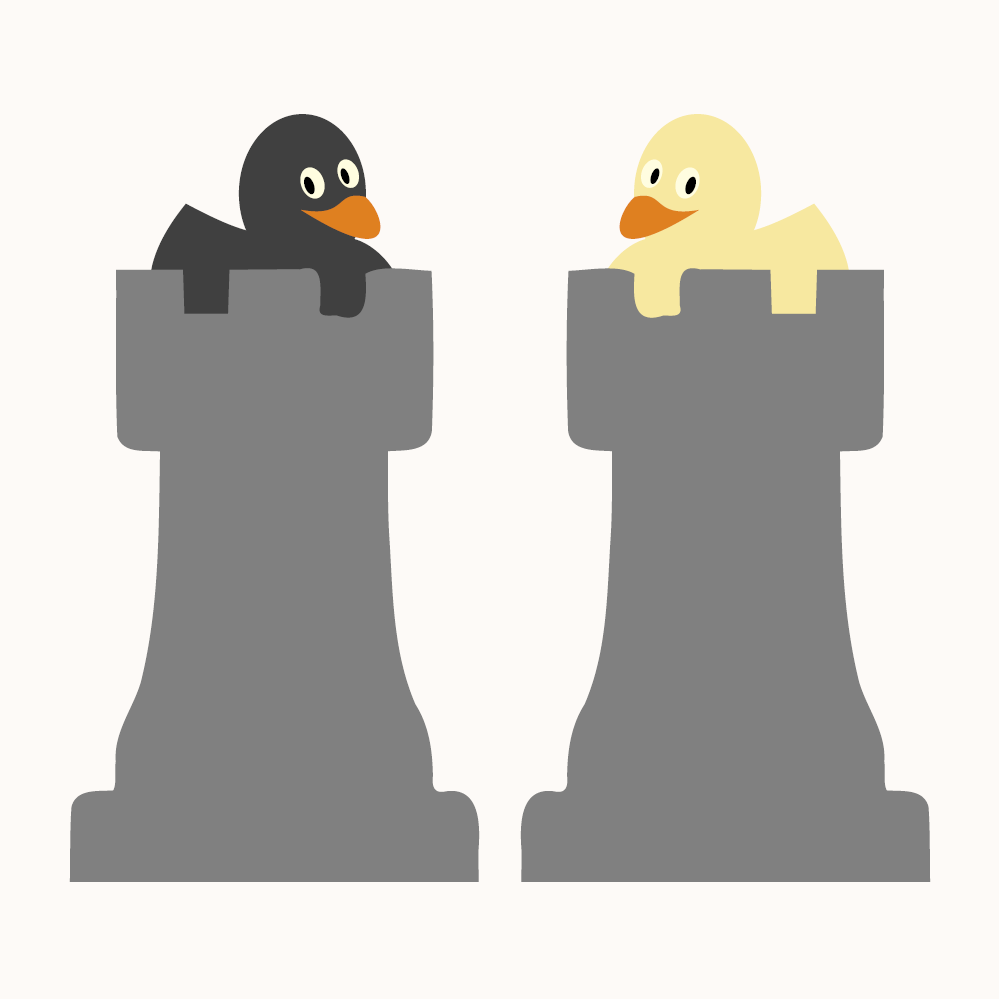
\includegraphics[width=0.8\linewidth,keepaspectratio]{ulrike-avatar}
&\vspace{-\ht\strutbox}
\includegraphics[width=0.75\linewidth,keepaspectratio]{carla-avatar}
\tabularnewline
\end{tabular}\\
\begin{tabular}{>{\centering}p{0.21\linewidth}>{\centering}p{0.20\linewidth}>{\centering}p{\dimexpr0.60\linewidth-6\tabcolsep}}

Screenplay  & Assistant &Cast \tabularnewline
\makebox[0pt][c]{Gert Fischer}      &Bär     &Loads of Tikzlings\tabularnewline
\vspace{-\ht\strutbox}
\includegraphics[width=0.8\linewidth,]{gert-avatar}
&\vspace{-\ht\strutbox}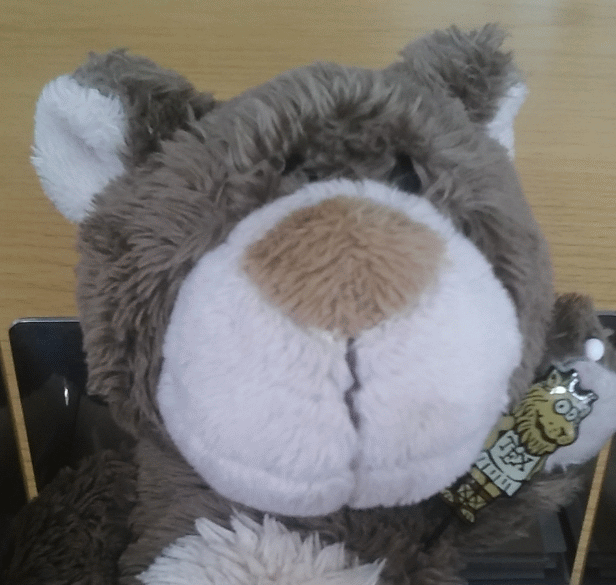
\includegraphics[width=0.8\linewidth,]{baer}&
\scriptsize\fontsize{6pt}{7.5pt}\selectfont\raggedright
\vspace{-2\normalbaselineskip}
Music and Sound by

...
\end{tabular}
\vfill\vfill
\end{document}
